\chapter{Stato dell'arte}\label{capitolo:arte}
\markboth{Stato dell'arte}{}

In questo capitolo di apertura vogliamo fornire una breve descrizione dei sistemi di \emulazione{} di reti di computers esistenti mettendoli a confrondo per capire le loro potenzialità; in parlicolar modo verrà descritto come questi si comportano davanti ad un utente che vuole creare configurazioni per reti complesse.

Nella seconda parte verranno discusse le qualità della prima release\footnote{Release, letteralmente ``rilascio'', in ambito informatico indica una particolare versione di un software resa disponibile ai suoi utenti, univocamente identificata da altre particolari versioni rese disponibili in precedenza da un particolare numero di versione.} di \visualnetkit{} e, come si vedrà nei successivi capitoli, verranno enfatizzati i punti deboli di questa prima versione che verrà messa a paragone con le pontenzialità offerte dal nuovo e più flessibile ambiente offerto dalla nuova release.

\section{Panoramica sui sistemi di \emulazione{}}
Prima di concentrare i nostri sforzi sul capire cosa rappresenta un ``ambiente di \emulazione{}'' focalizziamo l'attenziene sul significato stesso della parola \emulazione{}. Un software di \emulazione{} o più comunemente chiamato ``emulatore'' è un programma che permette l'esecuzione di software scritto per un ambiente (hardware o software) diverso da quello sul quale l'emulatore stesso viene eseguito.

Un programma scritto e compilato per una determinata piattaforma software (ad esempio \windows) non viene eseguito su un computer con sistema operativo differente come \linux{}. In questi casi si crea sulla macchina ospitante ``Host'' un emulatore che riproduce virtualmente l'ambiente che è stato usato per creare quel programma (nel nostro esempio un ambiente \windows{}). Il sistema virtuale che gira all'interno di quello emulato viene chamato sistema ``Guest''.

I sistemi di \emulazione{} di reti nascono con l'intento di riprodurre il funzionamento delle reti reali e di tutti i servizi che esse offrono agli utenti; configurazioni particolari, protocolli, ecc\ldots

Una rete di calcolatori può essere definita come un sistema informatico costituito da due o più calcolatori che, collegati tra loro tramite un mezzo trasmissivo, possono scambiarsi informazioni di vario genere. Naturalmente nella realtà le cose sono molto più complesse che una semplice definizione. Proprio per questo motivo un sistema di \emulazione{} deve offrire la possibilità di gestire qualsiasi configurazione e comportamento che i calcolatori presenti in rete possono assumere, permettendo così una rappresentazione eterogenea di macchine che offrono diversi servizi e svolgono diverse attività.

I sistemi attualmente esistenti permettono la creazione di reti composte da centinaia di computers generando, di conseguenza, un proporzionale aumento di macchine interfaccie di rete e protocolli coinvolti.

\subsubsection{Ma perché emulare reti di calcolatori?}
Lo scopo principale di un sistema di \emulazione{} di reti di calcolatori è quello di riprodurre e sperimentare il funzionamento dei nodi\footnote{Per ``nodo'' in una rete di calcolatori si intendono computers provvisti di memoria.} e dei connettori\footnote{Per ``connettore'' si intendono dispositivi come ad esempio hub, bridge, ecc\ldots}, al fine di testare nuovi protocolli e verificare il corretto funzionamento della rete. Tutto questo viene affrontato in maniera ``virtuale'' senza dover acquistare dispositivi spesso molto costosi.

Si pensi ad esempio all'ambito didattico; lo studente (o il ricercatore, o l'individuo che vuole studiare e sperimentare reti di calcolatori) dovrebbe dapprima studiare la soluzione ``su carta'', acquistare le dovute apparecchiature di rete (che come noto hanno un impatto economico non trascurabile), assemblare la rete, configurare adeguatamente ogni singolo nodo e connettore della rete e solamente alla fine passare alla fase di test sulla rete assemblata. E cosa succede se lo studente volesse modificare una parte della rete? Da questo si evince immediatamente che questo scenario nella maggior parte dei casi non è praticabile e come l'uso dei sistemi di \emulazione{} semplifichi notevolmente tali attività rendendo possibile l'intera progettazione su di un singolo calcolatore che ospita un sistema di \emulazione{}.


\subsection{Classificazione dei sistemi di \emulazione{}}
Allo stato attuale esistono molteplici tipologie di soluzioni offerte nel campo dell'\emulazione{} di sistemi. In questi ulmiti anni il bisogno di prototipi ed ambienti per la realizzazione di esperimenti nel campo delle reti di calcolatori ha catturato grande attenzione nel mondo della ricerca e dello sviluppo, dirottando notevoli sforzi in tal senso portando alla distinzione di tre principali classi di metodologie e strumenti: reti \testbed{}, \simulazione{}, \emulazione{} di reti e \virtualmachine.

Le reti \testbed{} sono ambienti costruiti su un hardware reale, come routers o hosts, interconnessi e propriamente configurati atti a realizzare la tipologia di rete desiderata. Sebbene questa soluzione è in grado di offrire un elevato grado di realismo, gli ambienti \testbed{} tendono ad essere difficilmente realizzabili per via dell'elevata difficoltà di realizzazione, mantenimento e soprattutto per costi talvolta proibitivi e raramente accessibili.

I simulatori offrono ambienti per la realizzazione di reti concettuali. Questi sono tipicamente stumenti altamente configurabili ed estensibili progettati per testare e valutare le dinamiche di rete in un ambiente disaccoppiato da ogni sorta di traffico o sistema esterno. 

Gli emulatori di reti (di cui ci occuperemo meglio più avanti) possono essere considerati un innesto di reti \testbed{} e simulatori di reti essendo in grado di riunire le caratteristiche proprie del traffico e dei sistemi coinvolti nelle reti reali. La maggior parte di essi, infatti, è costituito da un \emph{motore di emulazione} e di un interfaccia che permetta di interagire con lo stesso. Il motore dell'emulatore assolve il compito di mantenere in piedi il sistema emulato agendo a basso livello, spesso con primitive di sistema. Esso è in grado di riprodurre virtualmente tutte le componenti hardware e software, e quindi, di predisporre un ambiente standard ``gradito'' al sistema che si andrà ad emulare.

Le \virtualmachine{}, infine, si possono considerare un ``PC nel PC''. Ossia, mediante una \virtualmachine{} è possibile installare un secondo sistema operativo in una macchina virtuale e farci girare software in un ambiente considerato più ``protetto'' che non la macchina host vera e propria. Come si può immaginare, al di là della lentezza (comunque relativa e proporzionale alla potenza della macchina host), non vi è alcun limite. Questi sistemi a volte emulano anche parti di hardware, e altre volte si limitano a replicare l'hardware della macchina host. Una \virtualmachine{} solitamente è posizionata all'interno di un sistema di \emulazione{}. Quest'ultimo aspetto verrà ripreso più volte durante il corso del lavoro proposto.


\subsection{Ambienti di \emulazione{} a confronto}
Negli ultimi anni si sono affermati diversi strumenti ed ambienti di emulazione che possono essere caratterizzati sulla base delle tecniche di emulazione adottate, dei tipi di dispositivi da essi emulati o di licenza con cui sono distribuiti oltre che per le diverse funzionalità offerte.

Di seguito andremo a descrivere brevemente alcuni dei più rappresentativi in materia di emulazione di reti.

\paragraph{Imunes}\cite{OSSINI} è un software di emulazione che si avvale di una estensione del kernel \textit{FreeBSD} capace di eseguire più istanze indipendenti dello stack di rete su un unico kernel del sistema operativo. Un editor grafico della topologia di rete consente di preparare rapidamente esperimenti costituiti da apparati di rete quali hub, switch, router e host.
\begin{figure}[!ht]
	\centering
	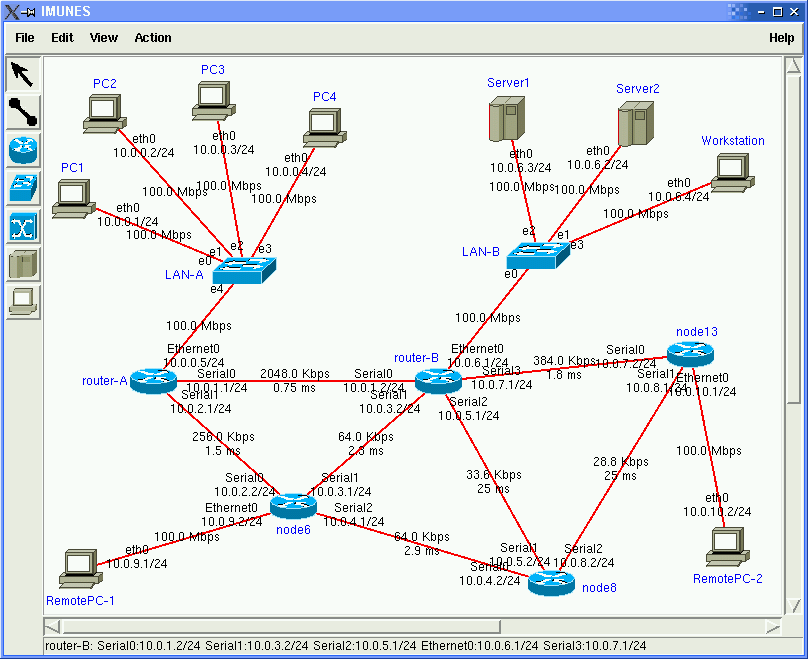
\includegraphics[width=9cm]{images/imunes_gui_normal.png}
	\caption{GUI per il software di emulazione IMUNES.}
	\label{figura:imunes_gui}
\end{figure}

\paragraph{Marionnet}\cite{MVNL08} è anch'esso un ambiente di emulazione di reti virtuali. Permette all'utente di definire, configurare ed istanziare reti di computer anche complesse senza alcun bisogno di apparati fisici. Scritto in \textit{OCaml} ed appogginadosi su \emph{User Mode Linux}\footnote{\emph{User Mode Linux} (UML) da la possibilità di avviare varie \virtualmachine{} con sistema \linux{} (sistema ``Guest'') per eseguire applicazioni come quello che accade con un normale sistema \linux{} (sistema ``Host''). Ogni sistema guest è una normale processo avviato in \emph{user space}.} e \textit{VDE}\footnote{VDE è un  rete virtuale compatibile con ethernet che può essere configurata su una rete di computer fisici su Internet. VDE fa parte del progetto \textit{VirtualSquare}.}, offre una interfaccia grafica molto intuitiva.
\begin{figure}[!ht]
	\centering
	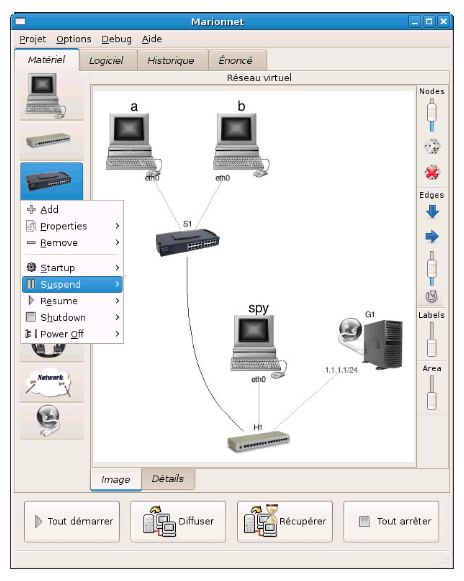
\includegraphics[width=9cm]{images/marionnet_gui.png}
	\caption{Finestra principale di Marionnet mostra una rete composta da tre computer, uno switch un hub ed un gateway.}
	\label{figura:marionnet_gui}
\end{figure}

\textit{Netkit}\cite{NETKIT}  e \textit{VNUML}\cite{VNUMLT} sono entrambi emulatori di medie dimensioni che utilizzano un kernel \emph{User Mode Linux} per eseguire diverse esperienze su reti emulate.
\paragraph{Netkit}In \textit{Netkit} una rete viene modellata come la connessione di macchine virtuali. Per la creazione di un lab è necessario creare un file di configurazione per il lab stesso, in cui si descrive la topologia della rete, e alcuni file per ogni virtual machine che si vuole connettere alla rete (fig. \ref{figura:netkit_lab_files}). A seguire viene riportato un esempio di file di configurazione in riferimento allo schema di rete in figura \ref{figura:netkit_lab_schema}.\\
L'interazione tra l'utente finale e le macchine virtuali è possibile per mezzo di una interfaccia a riga di comando (fig. \ref{figura:netkit_gui}). Poichè in Netkit la virtualizzazione è realizzata grazie all'uso di User-Mode Linux e poichè tale modalità richiede spesso di aver a che fare con comandi alquanto complessi, vengono forniti una vastità di script atti a semplificare l'interazione con il sistema e le macchine virtuali.

\begin{figure}[!ht]
	\centering
	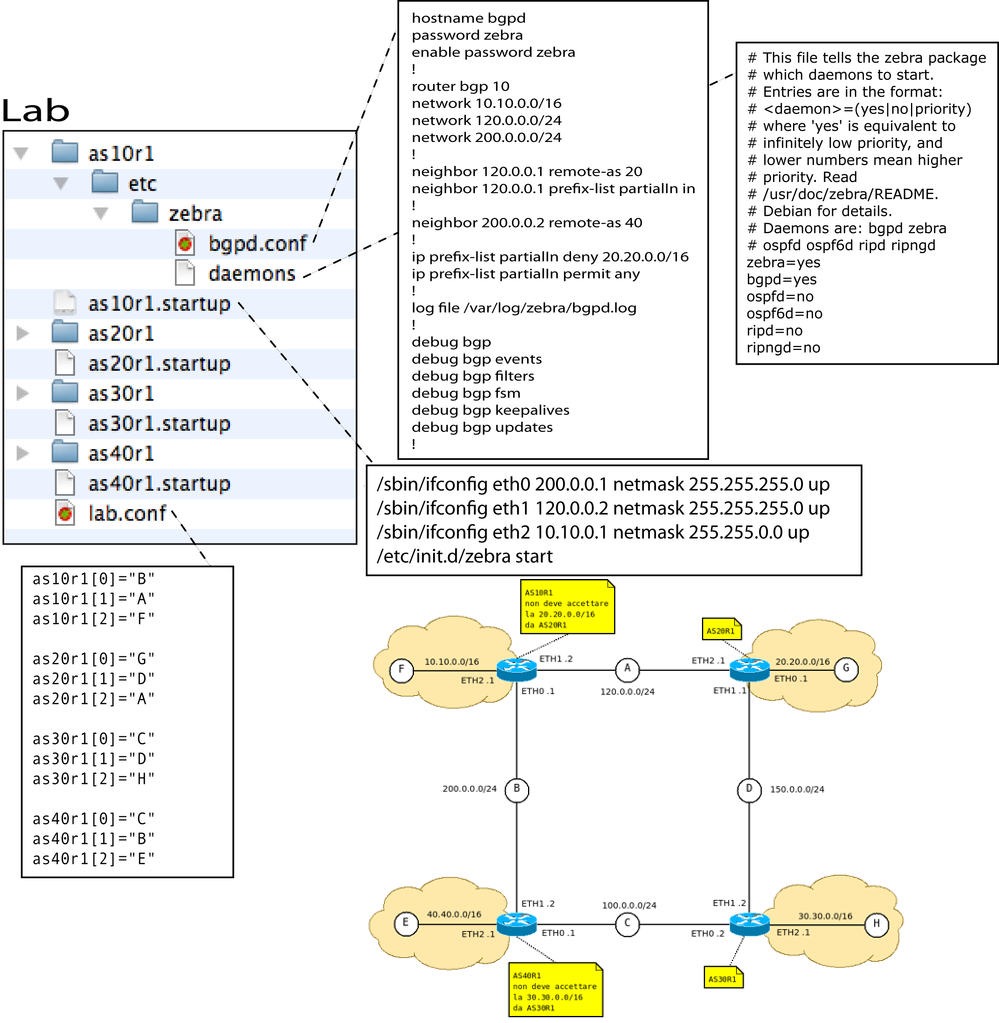
\includegraphics[width=9cm]{images/netkit_lab.png}
	\caption{Schema di rete di un semplice lab in Netkit.}
	\label{figura:netkit_lab_schema}
\end{figure}

\begin{figure}[!ht]
	\centering
	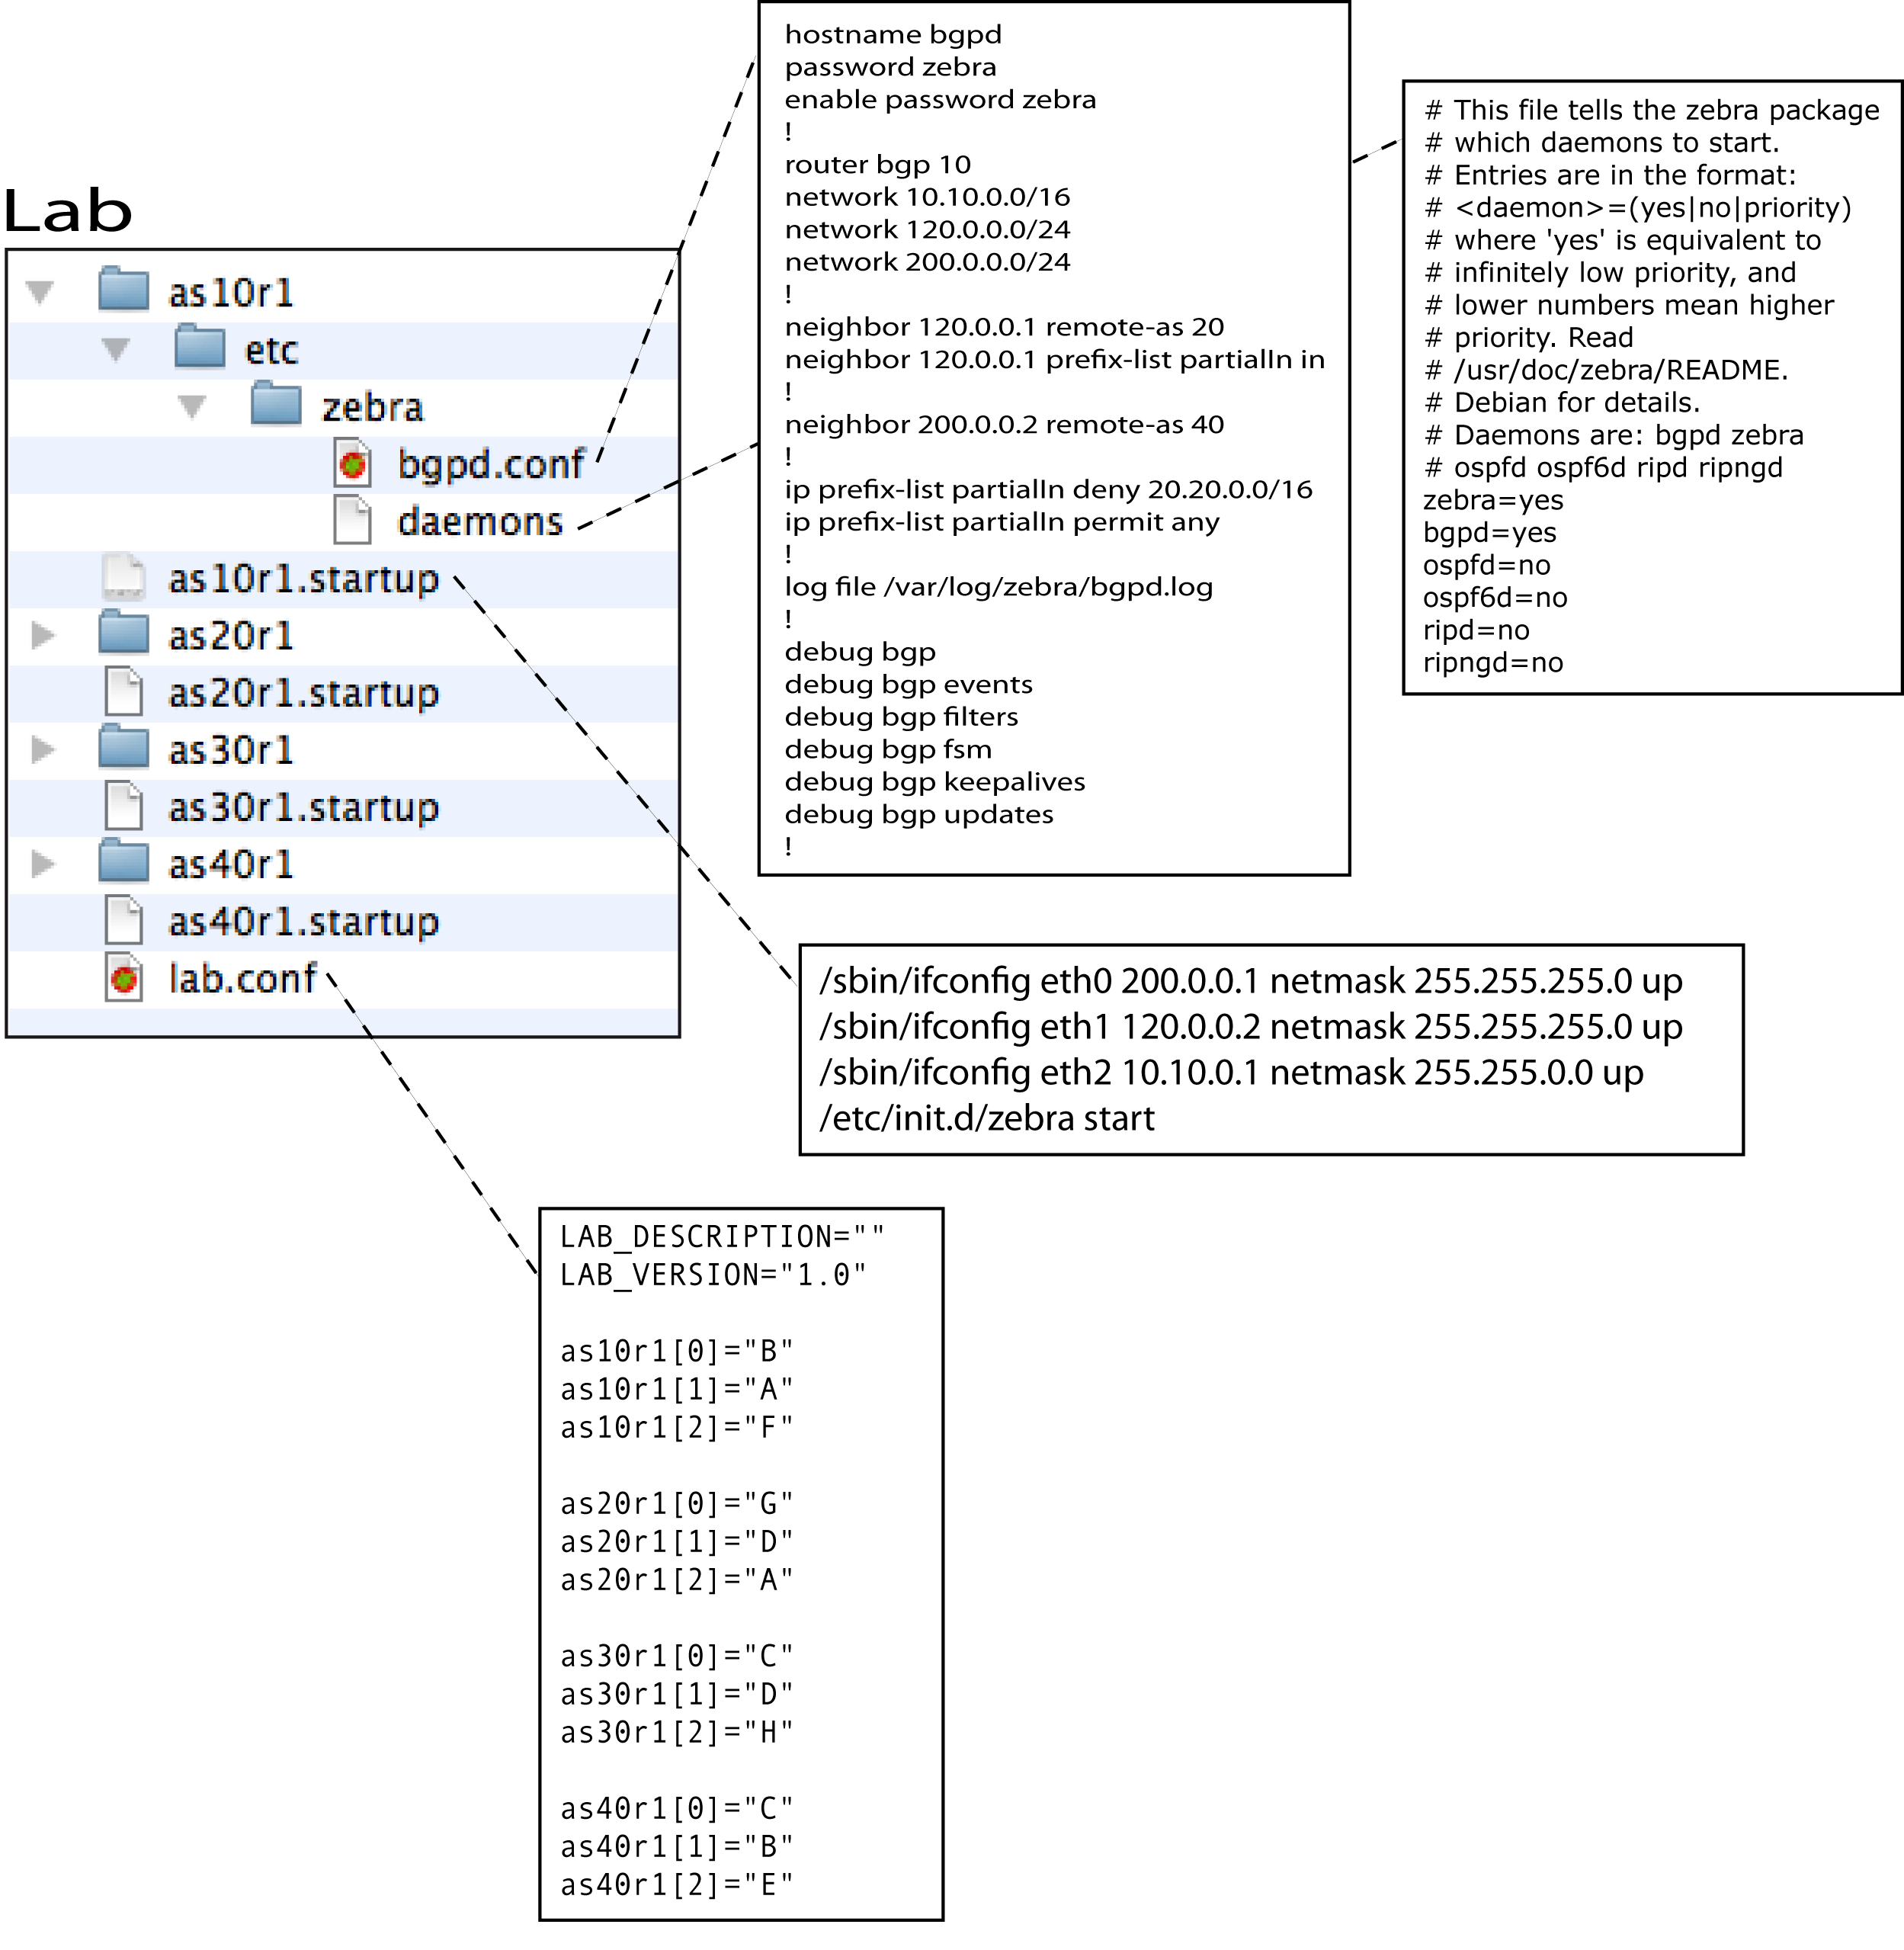
\includegraphics[width=9cm]{images/netkit_lab_files.png}
	\caption{Files di configurazione per il lab in figura \ref{figura:netkit_lab_schema}.}
	\label{figura:netkit_lab_files}
\end{figure}

\begin{figure}[!ht]
	\centering
	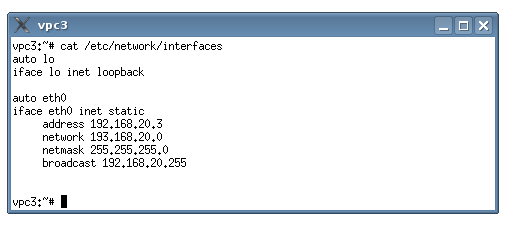
\includegraphics[width=9cm]{images/netkit_gui.png}
	\caption{UI per la configurazione di macchine virtuali in Netkit.}
	\label{figura:netkit_gui}
\end{figure}

\paragraph{Vnuml}\cite{VNUMLT} (Virtual Network User Mode Linux) è un ambiente di emulazione di reti che raccoglie una serie di script utilizzati per la descrizione di \testbed{} in XML, per il test di applicazioni di rete e servizi.\\
VNUML consiste in un linguaggio basato su XML, con una specifica sintassi, e di un interprete che può essere utilizzato per descrivere ed eseguire una rete emulata di macchine virtuali UML.\\
Dalla descrizione in XML degli scenari, VNUML istanzia le macchine virtuali UML e le configura. Nascondendo all'utente i dettagli avanzati e la configurazione virtuale delle macchine, questo ambiente risulta molto utile per testare scenari di rete anche complessi.\\Comunque, i progettisti devono descrivere il completo scenario di rete utilizzando il linguaggio XML che, a volte, richiede dettagli di rete molto specifici.\\
Ad affiancare questo ambiente allo scopo di introdurre una rappresentazione grafica intuitiva è stato realizzato \textit{VNUMLGUI}\cite{VNUMLGUI}. VNUMLGUI è un'interfaccia grafica per VNUML.\\
VNUMLGUI è soprattutto un editor di topologia con capacità grafiche. Permette di creare qualsiasi topologia di rete virtuale in VNUML senza dover editare manualmente il file XML ma con la sola immissione di router e interruttori.\\
Così come VNUML nasconde la curva di apprendimento di UML, VNUMLGUI nasconde la curva di apprendimento di VNUML e XML.

Di seguito sono riportati a titolo di esempio uno schema di rete e la sua corrispettiva implementazione in VNUML ed una raffigurazione dell'interfaccia grafica di VNUMLGUI.

\begin{figure}[!ht]
	\centering
	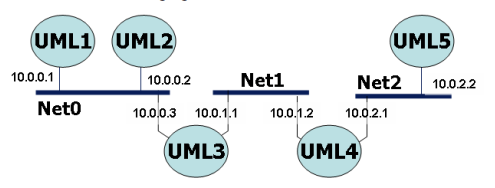
\includegraphics[width=9cm]{images/vnuml_01.png}
	\label{figura:vnuml_gui}
\end{figure}

\begin{scriptsize}
\begin{verbatim}
<?xml version="1.0" encoding="UTF-8"?>
<!DOCTYPE vnuml SYSTEM "/usr/share/xml/vnuml/vnuml.dtd">
<vnuml>
  <global>
    <version>1.7</version>
    <simulation_name>tutorial-lu</simulation_name>
    <automac/>
    <vm_mgmt type="none" />
    <vm_defaults>
       <filesystem type="cow">/usr/share/vnuml/filesystems/root_fs_tutorial</filesystem>
       <kernel>/usr/share/vnuml/kernels/linux</kernel>
       <console id="0">xterm</console>
    </vm_defaults>
  </global>
  <net name="Net0" mode="uml_switch" />
  <net name="Net1" mode="uml_switch" />
  <net name="Net2" mode="uml_switch" />
  <vm name="uml1">
    <if id="1" net="Net0">
      <ipv4>10.0.0.1</ipv4>
    </if>
    <route type="ipv4" gw="10.0.0.3">default</route>
  </vm>
  <vm name="uml2">
    <if id="1" net="Net0">
      <ipv4>10.0.0.2</ipv4>
    </if>
    <route type="ipv4" gw="10.0.0.3">default</route>
  </vm>
  <vm name="uml3">
    <if id="1" net="Net0">
      <ipv4>10.0.0.3</ipv4>
    </if>
    <if id="2" net="Net1">
      <ipv4>10.0.1.1</ipv4>
    </if>
    <route type="ipv4" gw="10.0.1.2">10.0.2.0/24</route>
    <forwarding type="ip" />
  </vm>
...
</vnuml>
\end{verbatim}
\end{scriptsize}

\begin{figure}[!ht]
	\centering
	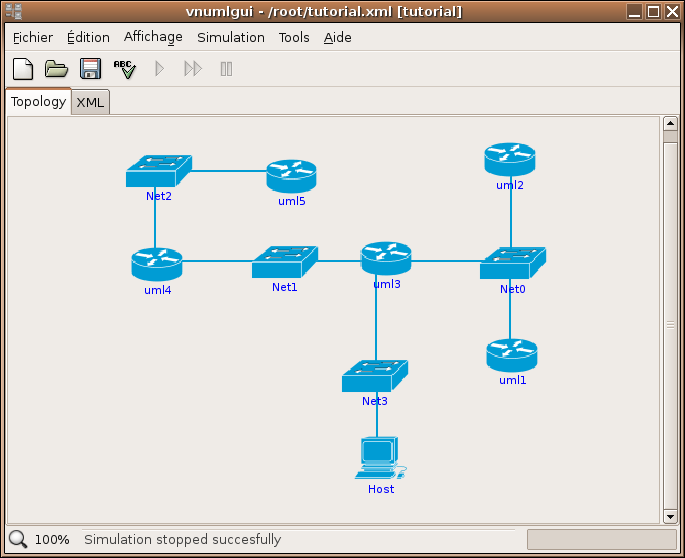
\includegraphics[width=9cm]{images/vnumlgui.png}
	\label{figura:vnumlgui}
\end{figure}

Sia Netkit che VNUML sono emulatori realizzati per offrire all'utente una rappresentazione ad alto livello della rete modellata. NETGUI e VNUMLGUI concretizzano tale scopo. Tutto ciò conferma l'intuizione che è dietro questo progetto e l'importanza di un supporto grafico facile da usare.

\paragraph{Qemu}\cite{QUATC05} è un emulatore e virtualizzatore di macchine che fa uso di una traduzione dinamica per ottenere una buona velocità di emulazione. QEMU offre due modalità operative: full system emulation ed user mode emulation, entrambe accessibili tramite interfaccia a riga di comando. Nella prima modalità, QEMU emula un sistema completo (ad esempio un PC), tra cui uno o più processori e le varie periferiche. Nella seconda modalità, QEMU può avviare processi compilati per una CPU su un'altra CPU.

QEMU è capace di simulare diverse VLAN. Una VLAN può essere rappresentata da un collegamento virtuale tra diversi dispositivi di rete. Questi dispositivi possono essere ad esempio schede Ethernet virtuali QEMU o dispositivi Ethernet su host virtuali.

\section{Ambienti di configurazioni a confronto}

\subsection{Creazione di configurazioni di reti complesse}

\subsubsection{Sistemi a confronto}

\subsubsection{Interfacce grafiche di supporto}

\subsubsection{Flessibilità delle interfaccie grafiche nei sistemi esistenti}

\subsubsection{La prima versione di \visualnetkit{}}


